\documentclass{scrartcl}


\usepackage{texenv}
%\usepackage{graphicx}
\begin{document}

%title
%\noindent\makebox[\linewidth]{\rule{\textwidth}{0.2pt}}
{\Large \centering \textsf{IT-Systeme: "Ubungsblatt 07} -- Florian Macherey, 
\today}\\
\noindent\makebox[\linewidth]{\rule{\textwidth}{0.2pt}} \\

%\normalsize \flushleft

\section*{Aufgabe 1: Bufferoverflows}
\subsection*{1a) Beschreiben Sie, was bei einem Bufferoverflow passiert?}
Bei einem Bufferoverflow wird die Puffergr"o\ss e ausgenutzt. Wenn der Puffer zu 
klein f"ur die Daten ist, werden die anderen Daten im Speicher "uberschrieben.

\subsection*{1b) Wo liegt die Gefahr von Bufferoverflows?} 
Wenn es zu einem Bufferoverflow kommt, ist die Gefahr eines Programmabruchs 
gro\ss ~. Entweder weil Variablen dann falsche Werte haben oder weil die 
R"ucksprungadresse von Funktionen nicht mehr korrekt ist. Dies f"uhrt dann zu 
einen Speicherzugriffsfehler (\textit{Segmentation Violation, SIGSEGV}). 

\subsection*{1c) Wie kann ein Bufferoverflow verhindert werden?}
Man kann Bufferoverflows verhindern, indem man Funktionen vermeidet, die bei 
Kopiervorg"angen nicht die Gr"o\ss e der Element "uberpr"ufen, wie zum Beispiel 
\texttt{fgets} in C. Au\ss erdem k"onnen Tools verwendet werden, die auf 
Betriebssyemebene ein "uberschreiben der R"ucksprungaddrese verbieten bzw. 
kontrollieren.

\section*{Aufgabe 2: XSS \\Vergleiche sie die Cross-Site-Scripting-Attacke mit einer SQL-Injection.}
\subsection*{2a) Welche Gemeinsamkeiten gibt es?}
\begin{itemize}
\item werden "uber Webanwendungen ausgef"uhrt
\item Manipulation des laufenden Systems 
\item Nicht expizit einzelne Nutzerinnen und Nutzer sind das Ziel
\end{itemize}

\subsection*{2b) Welche Unterschiede gibt es?}
\begin{itemize}
\item[\textit{XSS}] geziehlt Nutzerdaten stehlen bzw. nutzen 
werden
\item[\textit{XSS}] Angriff durch Scriptsprachen
\item[\textit{XSS}] Verschiede Aufrufe einer Seite
\item[\textit{XSS}] Angriff meist beim "ubergeben von Parameter an eine 
dynamische Webseite
\item[\textit{SQL-I}] das DBMS soll manipuliert werden
\item[\textit{SQL-I}] ein Aufruf einer Webanwendung
\end{itemize}

\section*{Aufgabe 3: Passwordcracking}
Quellcode zum Passwordcracking. Es wird ein Hybridverfahren verwendet, bei 
welchem zuerst h"aufig verwendete Passw"orter aus einen W"ortbuch ausprobiert 
werden, danach werden alle "ubrigen Kombinationen per Brute-Force ermittelt. 
Wenn ein Passwort bzw. sein Hashwert erfolgreich gefunden wurde, wird das 
Programm beendet, ohne die weitern M"oglichkeiten zu testen.

\lstinputlisting[language=Java,]{ue07.03/Encrypt.java}

\section*{Aufgabe 4: Bonusaufgabe \\Legen sie das Wort \dq Password\dq 
~aus Crackern und machen Sie ein Foto davon.}
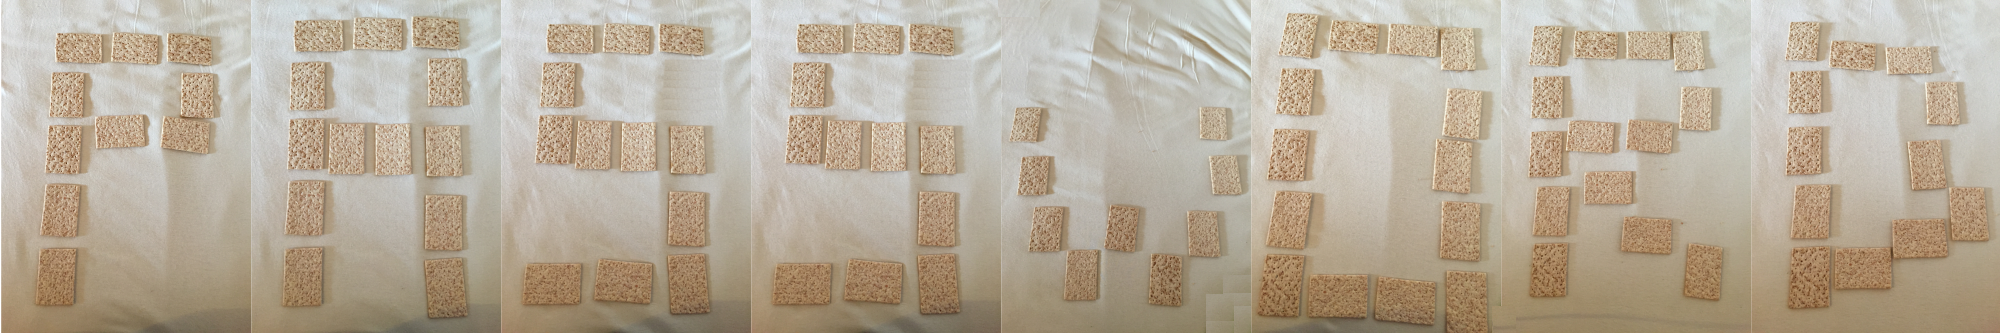
\includegraphics[width=\textwidth]{ue07-04-password.png}

\end{document}
